\documentclass[12pt]{article}

% Language setting
% Replace `english' with e.g. `spanish' to change the document language
\usepackage[spanish]{babel}

% Set page size and margins
% Replace `letterpaper' with`a4paper' for UK/EU standard size
\usepackage[a4paper,top=2cm,left=3cm,right=1.5cm,marginparwidth=1.75cm]{geometry}

% Useful packages
\usepackage{amsmath}
\usepackage{xcolor}
\usepackage{graphicx}
\usepackage[font=footnotesize,labelfont=bf]{caption}
\usepackage[allbordercolors=orange]{hyperref}
\usepackage{fontspec}
\usepackage{fancyhdr}
\usepackage{titling}
\usepackage{array}
\usepackage{multicol}
\usepackage{framed}
\usepackage{enumitem}
\usepackage[bibstyle=numeric, citestyle=numeric, sorting=nyt]{biblatex}
\usepackage{soul}
\usepackage{subcaption}
\usepackage{wrapfig}
\usepackage{listings}
\usepackage{layout}

\addbibresource{TIPPRA1.bib}

\definecolor{uocblue}{HTML}{000078}
\colorlet{main}{uocblue}
\setmainfont{Arial}[Color = uocblue]
\renewcommand{\labelitemi}{$\textcolor{uocblue}{\bullet}$}
\renewcommand{\labelitemii}{$\textcolor{uocblue}{\cdot}$}
\renewcommand{\labelitemiii}{$\textcolor{uocblue}{\diamond}$}
\renewcommand{\labelitemiv}{$\textcolor{uocblue}{\ast}$}
\renewcommand{\thefootnote}{\textbf{\arabic{footnote}}}
\renewcommand{\footnoterule}{{
		\color{uocblue}
		\kern 20pt
		\hrule width 2in
		\kern 3pt
}}
\setulcolor{uocblue}

\setcounter{biburllcpenalty}{7000}
\setcounter{biburlucpenalty}{8000}

\hypersetup{allcolors=uocblue}
\urlstyle{same}

% metadata
%%%%%%%%%%%%%%
\newcommand{\master}{Máster en Ciencia de Datos}
\newcommand{\grade}{2021/2022}
\newcommand{\subject}{Tipología y ciclo de vida del dato}
\newcommand{\testname}{\textbf{PRA1}}
\newcommand{\loginuocone}{agomezvarela@uoc.edu}
\newcommand{\loginuoctwo}{plazarotello@uoc.edu}
\newcommand{\authorone}{Alba Gómez Varela}
\newcommand{\authortwo}{Patricia Lázaro Tello}
\title{\textit{Web scraping} del mercado inmobiliario}
\author{Alba Gómez Varela\\Patricia Lázaro Tello}
\date{}	% quitar la fecha del titulo
%%%%%%%%%%%%%%

\pretitle{\vspace{-2cm}\begin{center}\LARGE \bfseries}
	\posttitle{\end{center}}
\preauthor{\vspace{-0.65cm}\begin{center}
		\large \itshape
		\begin{tabular}[t]{c}}
		\postauthor{\end{tabular}\end{center}\vspace{-1.5cm}}


\fancypagestyle{uoc}{
	\fancyhf{}
	\fancyhead[C]{
\includegraphics[width=16.5cm]{uoc.png}}
	\fancyhead[R]{\footnotesize \hspace*{\fill}\authorone \space \space · \space \nolinkurl{\loginuocone}\\
		\hspace*{\fill}\authortwo \space \space \space · \space\space\space \nolinkurl{\loginuoctwo}\\ \vspace{-2pt}}
	\fancyfoot[R]{\footnotesize \thepage} %\hspace{0.5cm}}
\fancyfoot[C]{\footnotesize \hspace{1.5cm} \grade}
\fancyfoot[L]{\footnotesize \subject \space · \testname\\
	\space\master}
\renewcommand{\headrulewidth}{0pt} % remove lines as well
\renewcommand{\footrulewidth}{0pt}
\setlength{\footskip}{50pt}%
\setlength{\headsep}{15pt}
\setlength{\headheight}{42pt}
\setlength{\parskip}{10pt}
\setlength{\topmargin}{-1cm}
%\setlength{\textheight}{\textheight}
\setlength{\textheight}{650pt}
\setlength{\oddsidemargin}{0pt}
\setlength{\marginparsep}{0pt}
\setlength{\marginparpush}{0pt}
\setlength{\voffset}{-10pt}
\setlength{\fboxsep}{0pt}
}

\pagestyle{uoc}
\linespread{1.125}
\color{uocblue}

\newlength{\leftbarwidth}
\setlength{\leftbarwidth}{0.15em}
\newlength{\leftbarsep}
\setlength{\leftbarsep}{0pt}
\renewenvironment{leftbar}{%
\def\FrameCommand{{\vrule width \leftbarwidth\relax\hspace {\leftbarsep}}}%
\MakeFramed {\advance \hsize -\width \FrameRestore }%
}{%
\endMakeFramed
}

\newenvironment{blockquote}{%
\par%
\leftskip=2em
%	\begin{leftbar}
	\noindent\ignorespaces}{%
	%	\end{leftbar}
\par}

\setlength{\parindent}{0em}

%%%%%%%%%%%
\definecolor{codegreen}{rgb}{0,0.6,0}
\definecolor{codegray}{rgb}{0.5,0.5,0.5}
\definecolor{codepurple}{rgb}{0.58,0,0.82}
\definecolor{backcolour}{rgb}{0.97,0.97,0.95}

\lstdefinestyle{mystyle}{backgroundcolor=\color{backcolour}, commentstyle=\color{codegreen},
keywordstyle=\color{magenta}, numberstyle=\tiny\color{codegray}, stringstyle=\color{codepurple},
basicstyle=\ttfamily\footnotesize, breakatwhitespace=false, breaklines=true, captionpos=t,                    
keepspaces=true, numbers=left, numbersep=5pt, showspaces=false,	showstringspaces=false,
showtabs=false, tabsize=4}

\lstset{style=mystyle}

\renewcommand*{\lstlistingname}{Documento}
%%%%%%%%%%%

\begin{document}

%\layout*

\maketitle
\thispagestyle{uoc}

%\vspace{-2em}
\begin{framed}
	\textbf{\underline{Houses for sale in the Salamanca and Villaverde district of Madrid in April 2022}}
	\begin{multicols}{2}
		\begin{itemize}[topsep=0cm,partopsep=0cm,label={},wide]
			\item \textbf{DOI}: \href{https://doi.org/10.5281/zenodo.6423459}{10.5281/zenodo.6418974}
			\item \textbf{Licencia}: CC BY-NC-SA 4.0
			\item \textbf{Número de registros}: 3.545
			\columnbreak
			\item 
\includegraphics[height=0.6cm]{zenodo.6423459}
			\item \textbf{Extracción}: 4-7 de abril de 2022
			\item \textbf{Número de campos}: 16
		\end{itemize}
	\end{multicols}
\end{framed}

\vspace{-2em}

\section{Contexto}\label{contexto}\vspace{-1.0em}

La \textbf{Ley por el Derecho a la Vivienda} se aprobó en España por decreto el 1 de febrero de 2022 y, aunque esta normativa no regula los pisos en venta ya construidos en la actualidad de forma directa, sí que podría afectar a su precio en el futuro. Por ejemplo, si se limita el precio del alquiler, se puede dar el caso de que los inversores dejen de estar interesados en estos bienes y, por tanto, el precio final de venta variaría al cambiar la demanda. Por otro lado, el 30\% de las nuevas promociones se reservará a Viviendas de Protección Oficial (VPO), lo que también puede alterar el precio de la vivienda libre.

Además de cambios en la normativa del mercado inmobiliario, la \textbf{invasión de Rusia a Ucrania} ha pillado por sorpresa a todos los sectores de la economía, disparando la \textbf{inflación} en España hasta un 9,8\%, según el indicador adelantado del IPC para el mes de marzo publicado por el Instituto Nacional de Estadística (INE). Del mismo modo, el Banco de España ha recortado sus \textbf{previsiones de crecimiento} para el país y ha doblado su previsión anual de inflación al 7,5\%, según los datos publicados el 5 de abril de 2022.

Asimismo, cabe destacar que el mercado inmobiliario en España se ha caracterizado desde hace décadas por las \textbf{diferencias en el precio} de la vivienda, tanto según las zonas del territorio nacional como dentro de las propias localidades. 

Teniendo presente esta situación de cambios económicos y normativos, y no existiendo un registro público de viviendas en venta actualizado, se ha decidido obtener la información de las viviendas en venta de los portales inmobiliarios de \textbf{Idealista} y \textbf{Fotocasa}. Esta decisión se fundamenta en que son los portales \textbf{más visitados} en España, según los datos de febrero de \href{https://www.similarweb.com/top-websites/spain/category/business-and-consumer-services/real-estate/}{\textit{\underline{similarweb}}}, que publica las métricas oficiales de los sitios web de todo el mundo. Además, esta clasificación de visitas se mantiene en los últimos años, por lo que no se prevé que varíe en un corto periodo de tiempo. Asimismo, es interesante que estos portales trabajan tanto con \textbf{inmobiliarias} como con \textbf{particulares} que desean vender inmuebles, por lo que proporcionan una información amplia sobre el tema de interés del proyecto.

%\begin{center}
%	\vspace{-0.5cm}
%	{\color{uocblue}\rule{0.75\linewidth}{1pt}}
%	\vspace{-0.5cm}
%\end{center}

\vspace{-1.5em}\section{Houses for sale in the Salamanca and Villaverde district of Madrid in April 2022}\vspace{-1.0em}

Debido a la gran cantidad de conjuntos de datos existentes sobre la temática seleccionada, para el \textit{dataset} resultante se ha optado por un título \textbf{muy descriptivo} a la par que \textbf{concreto}, de modo que solo con él se pueda saber el contenido del mismo. Además, debido a la volatilidad del mercado inmobiliario, se ha decidido incluir el mes de extracción de los datos.

%\begin{center}
%	\vspace{-0.5cm}
%	{\color{uocblue}\rule{0.75\linewidth}{1pt}}
%	\vspace{-0.5cm}
%\end{center}

\vspace{-1.5em}\section{Descripción del \textit{dataset}}\vspace{-1.0em}

El conjunto de datos obtenido a partir de los \textit{scrapers} hace referencia a todos los pisos disponibles durante la primera semana de abril de 2022 para su compra en los distritos de Villaverde y Salamanca en la ciudad de Madrid en los sitios web de Idealista y Fotocasa.

Se trata por tanto de una \textit{snapshot} del mercado inmobiliario en el distrito con el precio/m\textsuperscript{2} más bajo (Villaverde) y más alto (Salamanca) en Madrid. Con esta selección de distritos se busca descubrir las características que poseen los pisos de cada distrito, y si existe alguna otra razón, además del distrito en que se encuentra cada vivienda, que justifique su precio.

Cabe destacar que el conjunto de datos resultante no ha pasado por un proceso de limpieza, por lo que pueden existir inconsistencias en algunos campos; por ejemplo, los registros correspondientes a Fotocasa presentan el piso con un único número, mientras que en Idealista se muestran siguiendo el formato \verb|Planta {X}| (por ejemplo, ``Planta 1ª interior sin ascensor''). Otro ejemplo es el precio de los inmuebles, que en algunos casos se encuentra como \textit{string} con signos de puntuación.

El \textit{dataset} está guardado con codificación \textbf{UTF-8}, y cada registro se puede identificar inequívocamente mediante el par \verb|{id, source}|.

\vspace{-1.5em}\section{Representación gráfica}\vspace{-1.0em}

A continuación se muestra el flujo de este proyecto:

\begin{figure}[h]
	\centering
	\captionsetup{font={normalsize}}
	\fbox{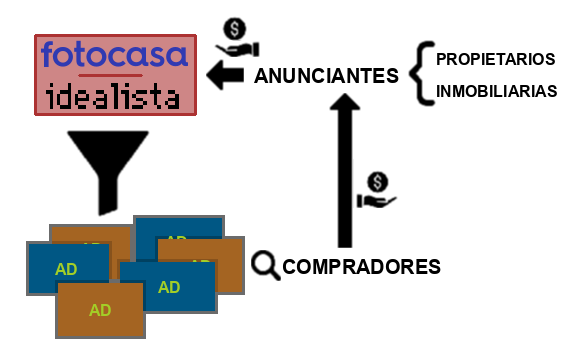
\includegraphics[width=\linewidth]{graphical-representation}}
	\caption{Representación gráfica del proyecto hasta llegar al \textit{dataset} final}
\end{figure}

Los \textbf{anunciantes}, que pueden ser tanto propietarios particulares como inmobiliarias, utilizan los portales de compraventa en el mercado inmobiliario para difundir sus \textbf{anuncios} de inmuebles. Por la creación de un anuncio, los \textbf{portales cobran} una tasa y la encarecen por otros servicios adicionales, como ocultar la dirección concreta en el caso de Fotocasa o promocionar o destacar el anuncio.

Los portales inmobiliarios ponen a disposición de los \textbf{compradores} dichos anuncios y ayudan a ponerles en contacto con los anunciantes, con los que cerrarán el trato fuera del portal.

En \textbf{este proyecto} se analizan dichos portales inmobiliarios y se vuelca en el \textit{dataset} final la información de los anuncios sobre \textbf{viviendas en venta} en \textbf{Fotocasa e Idealista}, en concreto de los distritos de \textbf{Villaverde} y \textbf{Salamanca} de Madrid, como ya se ha explicado en apartados anteriores. El resultado es un \textbf{CSV} con un registro por cada una de dichas viviendas y sus \textbf{planos} incluidos en los anuncios de Idealista, mientras que si el anuncio es de Fotocasa se han descargado todas las \textbf{fotografías} al carecer de la opción específica del plano. 

\vspace{-1.5em}\section{Contenido}\vspace{-1.0em}

%Explicar los campos que incluye el dataset, el periodo de tiempo de los datos y cómo se han recogido

Los datos han sido obtenidos durante la primera semana de abril de 2022 (del 4 al 7 de abril) de los portales inmobiliarios Idealista y Fotocasa. Los registros obtenidos representan la mayor parte de las viviendas en venta en los distritos Villaverde y Salamanca en la ciudad de Madrid.

\begin{figure}[h]
	\centering
	\captionsetup{font={normalsize}}
	\caption{Distritos de Villaverde y Salamanca \textit{scrapeados}}
	\begin{subfigure}{0.5\textwidth}
		\centering
		\fbox{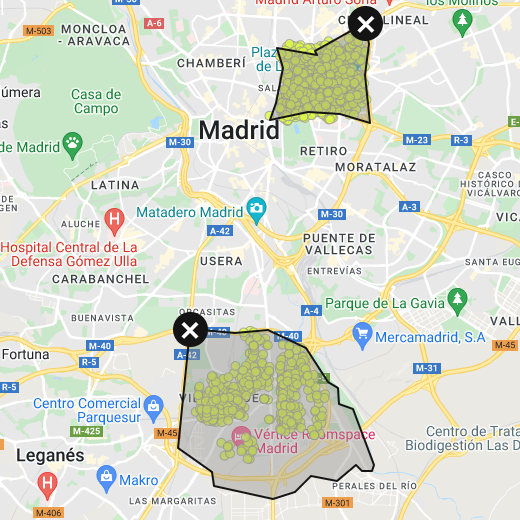
\includegraphics[width=\linewidth]{idealista-villaverde-salamanca}}
		\caption{\vspace{1.5em}Idealista}
	\end{subfigure}%
	\begin{subfigure}{0.5\textwidth}
		\centering
		\fbox{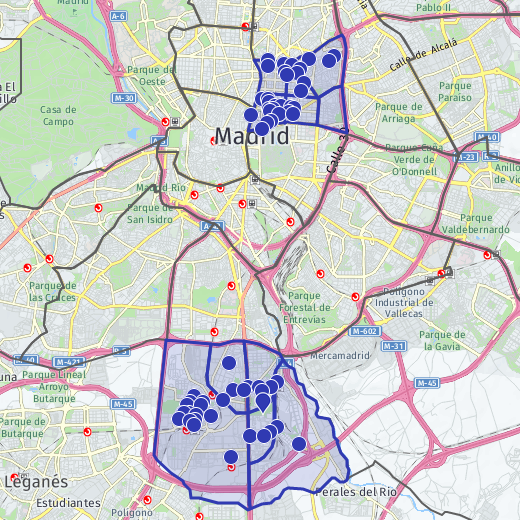
\includegraphics[width=\linewidth]{fotocasa-villaverde-salamanca}}
		\caption{\vspace{1.5em}Fotocasa}
	\end{subfigure}
	\vspace{-2.5em}
\end{figure}

Para obtener los datos se han utilizado las siguientes tecnologías:

\begin{multicols}{3}
	\begin{itemize}[topsep=0cm,partopsep=0cm,wide]
		\item Python 3.9.10
		\item Selenium 4.1.3
		\item BeautifulSoup 4.10.0
	\end{itemize}
\end{multicols}\vspace{-10pt}

Los datos se han obtenido mediante \textit{web scraping}. Se ha empleado principalmente \textbf{Selenium} por ser la tecnología que mejor imita el comportamiento humano al navegar por la web, aunque también se ha utilizado \textbf{BeautifulSoup} para comprobar los códigos de error cuando la página no cargaba según lo previsto.

Para optimizar los tiempos de ejecución, el proyecto se beneficia de las \textbf{características multihilo} que ofrece Python: por un lado, cada \textit{scraper} se lanza en su propio hilo \textemdash es decir, el \textit{scraper} de Fotocasa y el de Idealista se ejecutarán en paralelo \textemdash y a su vez, cada \textit{scraper} utiliza varios hilos para paralelizar el trabajo.

\begin{figure}[h]
	\centering
	\captionsetup{font={normalsize}}
	\fbox{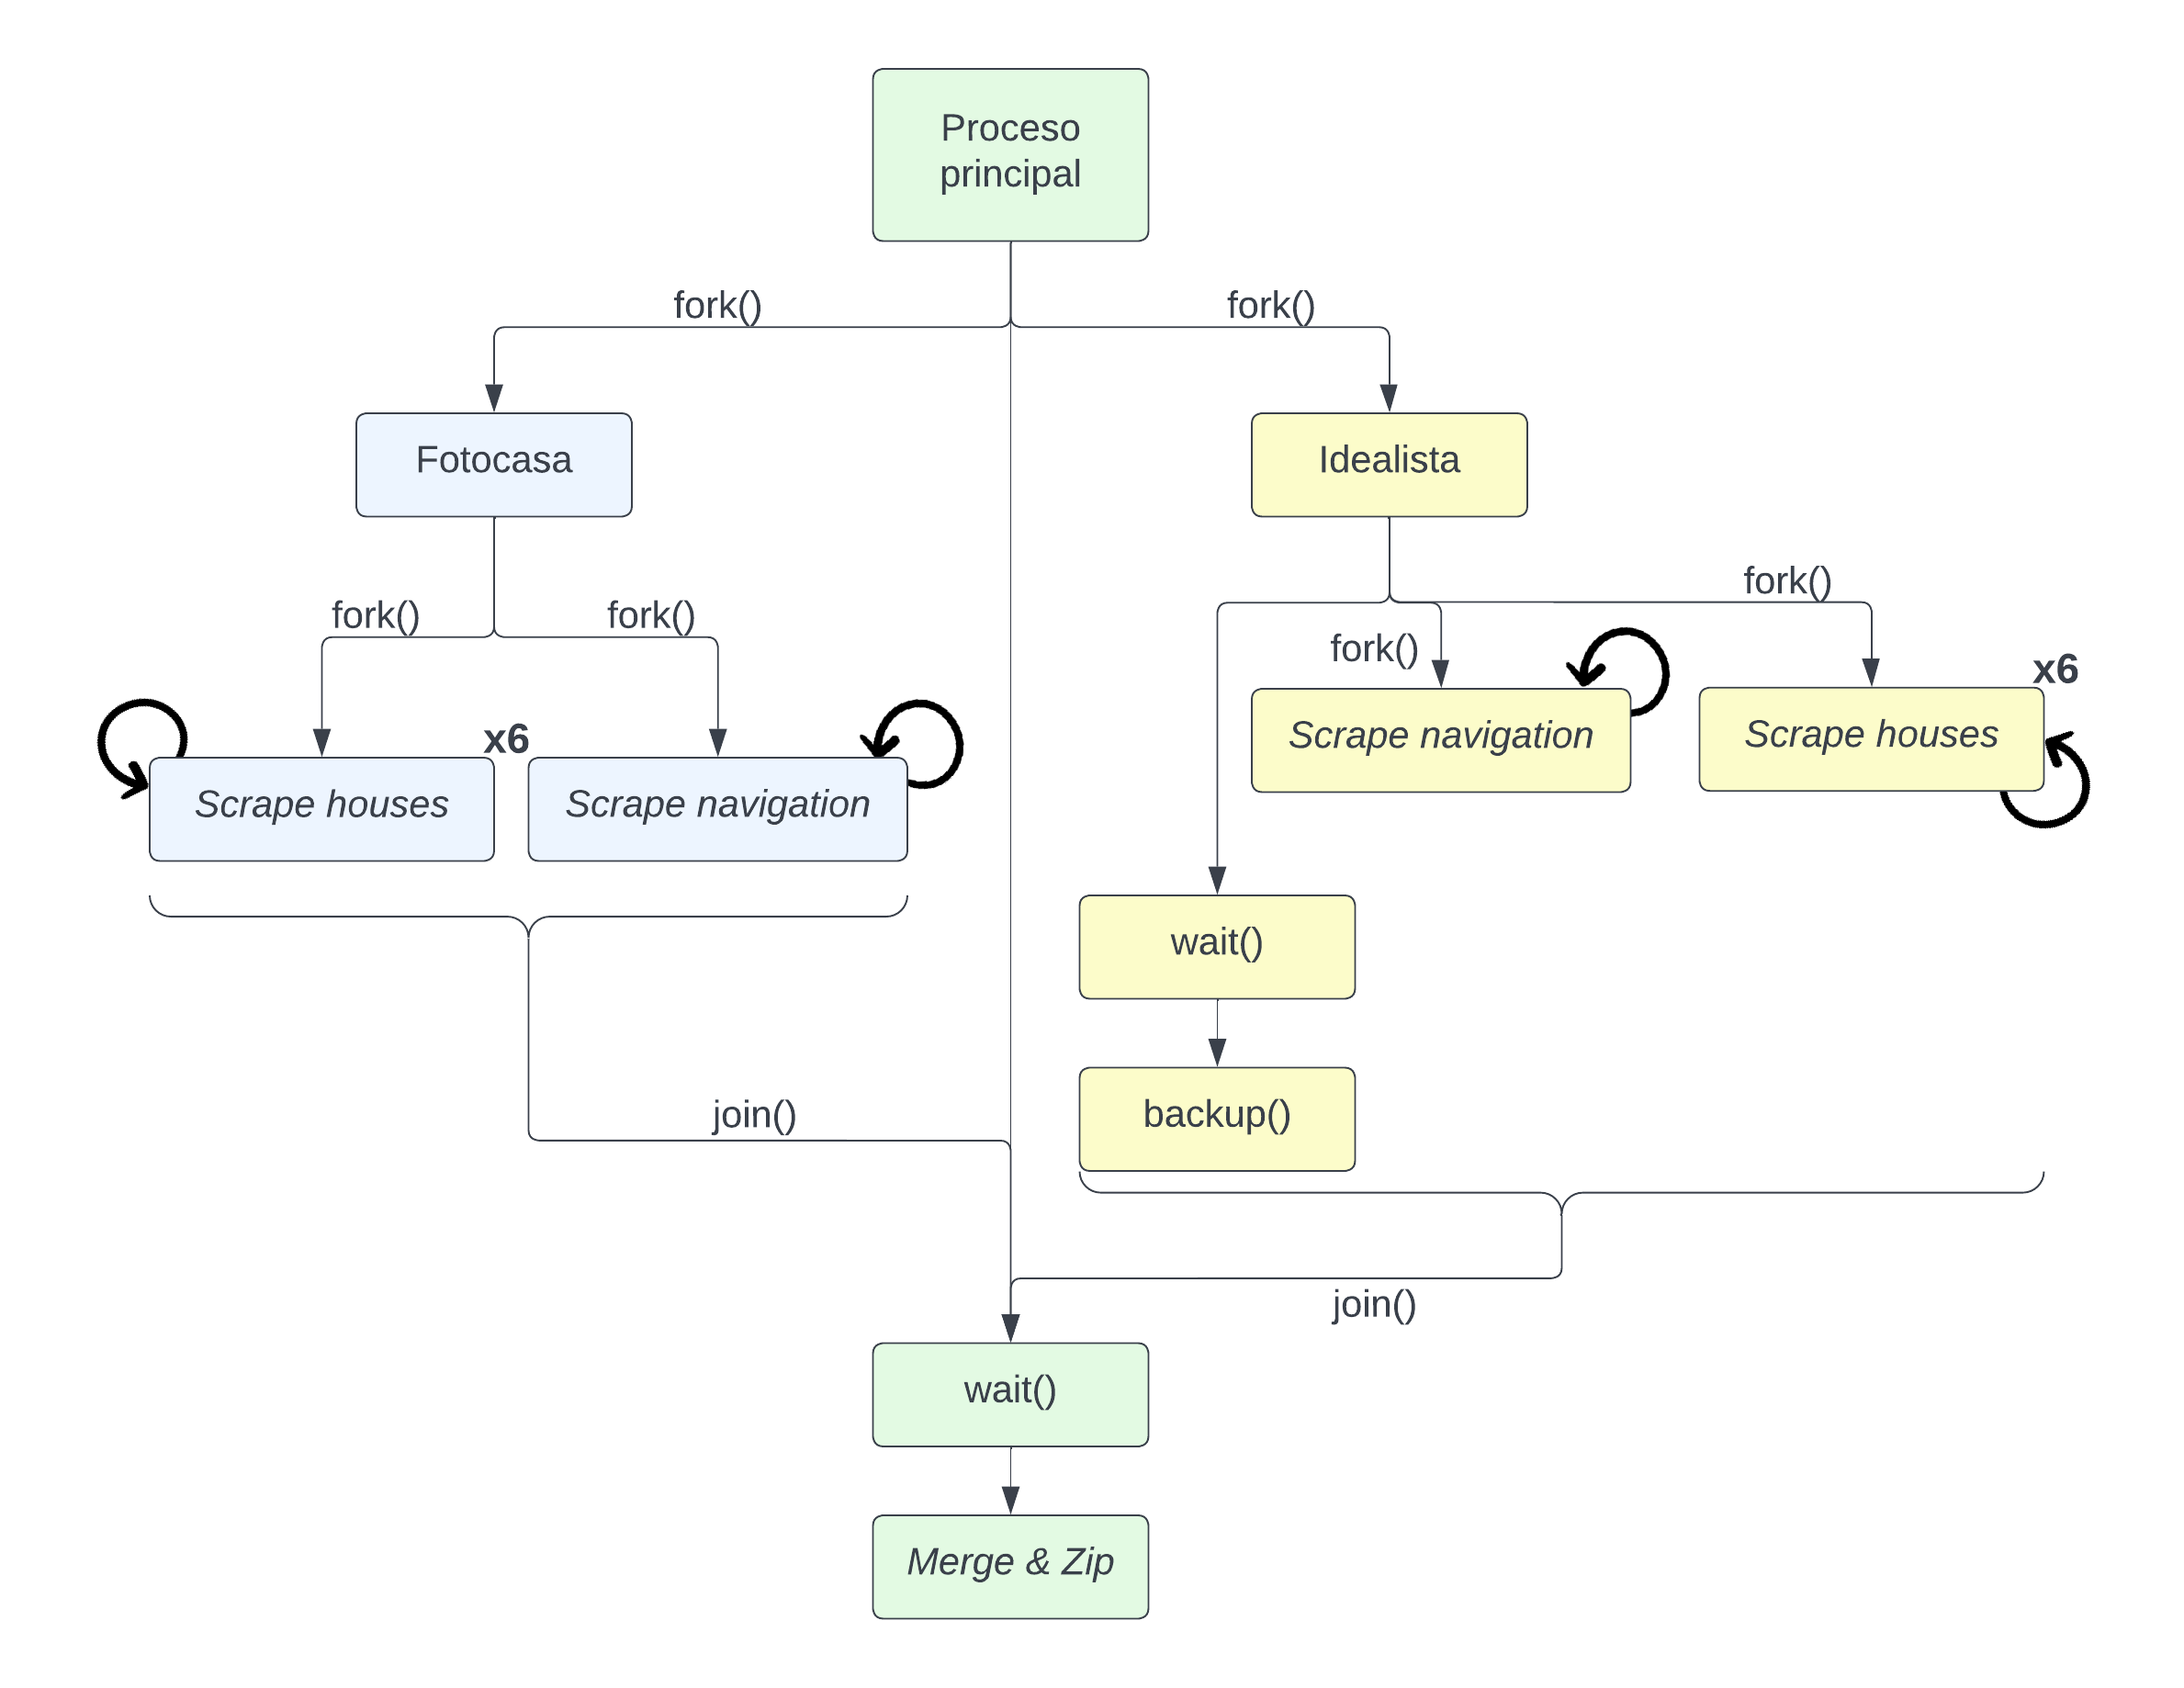
\includegraphics[width=\linewidth]{multithread}}
	\caption{\vspace{1.5em}Hilos de ejecución del programa y \textit{scrapers}}
	\vspace{-2em}
\end{figure}

Por otro lado, se han utilizado esperas activas, resolución automática de \textit{captchas} y técnicas de camuflaje mediante \textit{proxies} y cambios de \textit{user agent} del navegador de Selenium.

\newpage
Respecto a las \textbf{esperas activas}, esta ha sido la técnica que mejor ha funcionado para evitar ser bloqueados por Fotocasa e Idealista, pero como punto negativo añade retardos considerables al tiempo de ejecución de los \textit{scrapers} y no es efectiva al 100\% en Idealista.

Dada la limitada efectividad de las esperas activas en Idealista, se ha utilizado una \textbf{extensión gratuita para Google Chrome de resolución automática de \textit{captchas}} (\textit{Buster: Captcha Solver for Humans}), tampoco 100\% efectiva. Una alternativa consistente sería utilizar una extensión de pago de resolución de \textit{captchas}, pero no se ha considerado por estar fuera del presupuesto del proyecto.

También se han llevado a cabo acciones para camuflar las peticiones tan repetitivas del \textit{scraper}, con efectividad muy limitada. Por un lado, los \textbf{cambios de \textit{user agent}} no produjeron ningún efecto en Idealista para evitar la aparición de \textit{captchas} dado que este portal utiliza la IP del navegador para el conteo de peticiones. Sin embargo, la definición de un \textit{user agent} válido y la \textbf{desactivación de la opción \textit{headless}} en el navegador de Selenium evitó ser bloqueados en la primera petición a los portales.

Por otro lado, se probó la \textbf{utilización de \textit{proxies}} para evitar los bloqueos en Idealista, utilizando \textit{proxies} gratuitos disponibles en internet. Esta técnica, sin embargo, no terminó de ocultar la IP de la petición, por lo que no surtió ningún efecto. Sin embargo, es posible que con \textit{proxies} de mayor calidad y, por tanto, de pago, se hubiera conseguido un resultado mucho más favorable. Finalmente, se optó por no utilizar \textit{proxies} debido al retardo añadido a las peticiones del servidor, aunque se ha dejado esta posibilidad en el proyecto por si se quisiera retomar como opción en el futuro.

\vspace{-1.5em}\subsection*{Detalles del \textit{scraper} de Fotocasa}\vspace{-1em}

El primer reto solventado en el portal inmobiliario \textbf{Fotocasa} es el de la aceptación de las \textit{\textbf{cookies}}, sin lo cual no se puede navegar libremente por el portal. Por ejemplo, no permite cambiar de página y, por tanto, extraer la URL de todos los inmuebles en venta en una zona. Para saltar esta barrera, y gracias a Selenium, tras cargar la página con las viviendas por ubicación se simula el clic sobre la opción de aceptar dichas \textit{cookies}. Por otro lado, como al abrir cada URL de cada inmueble no afecta en nada no aceptar estas condiciones, en este otro caso no se hace para no añadir retardos al proceso de \textit{scraping}.

Además, Fotocasa cuenta con un sistema de \textbf{carga diferida} o \textit{\textbf{lazy loading}} tanto en las páginas que ofrecen los listados de los inmuebles como en las URL de las casas en sí mismas. Esto se traduce en que los contenedores o \textit{div} con la información de cada página se van cargando a medida que aparecen en la sección visible del navegador, es decir, conforme el usuario va navegando hacia abajo por la página (\textit{scroll}).

Así, esta carga diferida supuso un reto a la hora de obtener la información general de cada inmueble mediante el \textit{scraping} de las páginas de navegación y de las fotografías en las URL de las casas, ya que la información no se puede descargar tras la carga. El desafío, en este sentido, fue identificar el problema ya que el portal lo maneja de forma transparente el usuario y solo se encontró  mediante depuración en un navegador aparte. Se soluciona empleando Selenium para emular el comportamiento humano de hacer \textit{scroll} hacia abajo, de manera que se puedan cargar de forma asíncrona todos los elementos de dicha página.

Otro obstáculo solventado es que \textbf{las clases} y, en ocasiones, los \textbf{\textit{div}} en los que se aloja la información de cada inmueble en las páginas que muestran los listados de resultados según la ubicación no son los mismos. Esto quiere decir que la estructura del portal cambia a medida que se avanza por estos listados a través de las diferentes páginas de una misma ubicación, progresión que también se hace simulando un clic sobre el botón de \textit{página siguiente} emulando el comportamiento humano con Selenium. 

Para saltar la traba de la estructura variable, que provocaba que solo se pudiera almacenar información del 8\% de los inmuebles, se opta por evaluar la ubicación a \textit{scrapear} en cada caso, de manera que el programa ya detecta cuál es la estructura prevista debido a que se ha adaptado el código a cada una de ellas.

\vspace{-1.5em}\subsection*{Detalles del \textit{scraper} de Idealista}\vspace{-1em}

El portal inmobiliario \textbf{Idealista} cuenta con un sistema de bloqueos para \textit{bots} utilizando \textit{captchas} para evitar sus peticiones. Este fue el principal escollo en el diseño del \textit{scraper}, y como se explica en esta misma sección, se solucionó parcialmente mediante cambios de \textit{user agent}, la utilización de un \textit{captcha solver} gratuito y esperas activas (no se utilizaron \textit{proxies} finalmente dado que apenas producían beneficio pero introducían grandes retardos en el sistema de \textit{scraping}).

Debido a todas las salvaguardas para evitar la detección de Idealista, el \textit{scraper} de este portal inmobiliario dedica mucho tiempo a las esperas activas, dilatando en gran medida el tiempo requerido para obtener toda la información del sitio web. 

Una consecuencia de que la ejecución completa del programa se extienda tanto en el tiempo es que la fase de pruebas es muy costosa. Así mismo, si sucede un error inesperado (dentro o fuera del programa) y el \textit{scraper} se bloquea, el coste también es muy grande.

Teniendo estas consideraciones en mente, se ha decidido implementar un sistema de recuperación (\textit{backup}) y reanudación del \textit{scraping} mediante una sincronización cada \verb|X| \textit{links} visitados.

El \textbf{proceso de sincronización} utiliza un sistema de semáforos y eventos para controlar el número de páginas visitadas por el \textit{scraper} de navegación los \textit{scrapers} de inmuebles; para poder obtener una nueva página que visitar, los procesos tienen que pedir turno primero al semáforo, que solo tiene \verb|X| huecos disponibles. Una vez los huecos del semáforo se acaban, los procesos avisan al evento y se ponen a la cola para poder obtener un nuevo \textit{link} cuando haya hueco disponible.

El proceso principal espera a que se lance el evento para comenzar su procedimiento de sincronización: primero espera a que los procesos en curso queden a la espera de nuevos turnos en el semáforo, luego lanza el sistema de recuperación y reanudación, y finalmente libera los huecos del semáforo y da el evento como procesado y terminado.

Este \textbf{sistema de recuperación y reanudación} funciona de tal manera que se guardan en disco y se recuperan unos objetos de estado, concretamente una lista de los \textit{links} de navegación que quedan por visitar, una lista de los \textit{links} de inmuebles por visitar y una lista de la información de los inmuebles que hay que guardar en disco en la próxima sincronización.

Para evitar que la memoria RAM se llene antes de que el \textit{scraping} se haya completado \textemdash este es uno de los errores que pueden suceder, que la máquina se quede sin memoria para cargar más páginas \textemdash, solo se guarda la información de los inmuebles que no se encuentra ya salvada en disco en el fichero CSV. Cuando se realiza la sincronización, además de guardar un \textit{pickle} de los objetos de estado se actualiza también el fichero CSV volcando la nueva información y liberando la memoria RAM asociada.

\vspace{-1.5em}\subsection*{Descripción de los campos del \textit{dataset}}\vspace{-1em}

A continuación se procede a describir los distintos campos del conjunto de datos final obtenido del \textit{scraping} de Fotocasa e Idealista. Se trata de un \textit{dataset} de 16 campos con 3.545 registros, que ocupa en total 9.8MB en disco. Cada registro puede identificarse de forma única mediante el par \verb|(id, source)|.

\begin{itemize}[topsep=0cm,partopsep=0cm]
	\setlength\itemsep{-0.5em}
	\item \textbf{\textit{id}}: entero con el identificador numérico del inmueble, dado por Idealista o Fotocasa.
	\item \textbf{\textit{source}}: cadena de texto que identifica la fuente de la que se ha obtenido la información del inmueble (\verb|"fotocasa"/"idealista"|).
	\item \textbf{\textit{url}}: cadena de texto con la dirección de la página web de la que se ha obtenido la información del inmueble.
	\item \textbf{\textit{title}}: cadena de texto con el título del anuncio del inmueble.
	\item \textbf{\textit{location}}: cadena de texto con el barrio al que pertenece el inmueble \\ (\verb|"barrio-de-salamanca"/"villaverde"|).
	\item \textbf{\textit{price}}: entero o cadena de texto con el precio del inmueble fijado en el anuncio.
	\item \textbf{\textit{m2}}: entero con los m\textsuperscript{2} (metros cuadrados) del inmueble.
	\item \textbf{\textit{rooms}}: entero con el número de habitaciones del inmueble. El campo puede estar vacío.
	\item \textbf{\textit{floor}}: cadena de texto con el piso o planta del inmueble. Puede contener información adicional, como por ejemplo si se trata de un inmueble con ascensor o una orientación interior o exterior.
	\item \textbf{\textit{num-photos}}: entero con el número de fotografías disponibles en el anuncio.
	\item \textbf{\textit{floor-plan}}: entero que representa si el anuncio cuenta con un plano del inmueble (\verb|1|) o no (\verb|0|).
	\item \textbf{\textit{view3d}}: entero que representa si el anuncio cuenta con una vista en 3D del inmueble (\verb|1|) o no (\verb|0|).
	\item \textbf{\textit{video}}: entero que representa si el anuncio cuenta con un vídeo que muestra el inmueble (\verb|1|) o no (\verb|0|).
	\item \textbf{\textit{home-staging}}: entero que representa si el anuncio cuenta con la característica de \textit{home staging} (\verb|1|) \textemdash muestra cómo quedarían algunas habitaciones del inmueble con otro estilo, cambiando muebles, etcétera \textemdash  o no (\verb|0|).
	\item \textbf{\textit{description}}: cadena de texto con la descripción del anunciante para el inmueble.
	\item \textbf{\textit{photo\_urls}}: lista con las direcciones de las fotografías del inmueble anunciado.
\end{itemize}

Además del CSV, como se ha señalado en secciones anteriores, se han descargado todos los \textbf{planos} incluidos en las viviendas de los anuncios de Idealista. Al carecer de esta posibilidad en Fotocasa, se opta por la descarga de todas las \textbf{fotografías} del anuncio. Este material audiovisual tiene restricciones de \textbf{\textit{copyright}}, por lo que no se ha publicado en Zenodo, pero sí a la carpeta privada de Google Drive. 

\vspace{-1.5em}\section{Agradecimientos}\vspace{-1.0em}

A continuación, se aborda el apartado de agradecimientos divido en tres bloques debido a la complejidad del proyecto planteado y a la necesidad de diferenciar claramente entre ellos. 

\vspace{-1.5em}\subsection*{Propietarios de los datos}\vspace{-1.0em}

Como se ha indicado en otros apartados, este es un proyecto en el que se integran \textbf{dos fuentes de datos} diferentes, con sus respectivos propietarios de los datos. 

Por un lado, sobre el portal web \href{http://www.idealista.com}{\textbf{\underline{Idealista}}}, cuyo fundador y CEO es Jesús Encinar, es importante destacar que la empresa está registrada como una Sociedad Anónima Unipersonal (Idealista S.A.U.) fundada en el año 2000, aunque en la actualidad está participada mayoritariamente por los fondos gestionados por EQT. En estos momentos, opera además en Portugal e Italia, países en los que no se centra este proyecto, pero cuya estructura de la web es idéntica, con todo lo que esto implica. 

Explorando el dominio mediante \textit{whois} de python, se obtienen otros datos del mismo, como que su fecha de creación fue el 21 de agosto de 1999 y otra información irrelevante en este punto.

Por otro lado, según explican ellos mismos y se puede verificar en gran medida en el desarrollo del código, el \textbf{desarrollo de software} de Idealista usa como base el sistema de arquitectura LEMP (Linux, Nginx, MySql, PHP) además de otras herramientas, como bases de datos (Oracle y SQLite), motores de búsqueda fulltext (Sphinxsearch y Solr), lenguajes de programación PHP en sus versiones 5.6 y 7.1 ó JavaScript, y Laravel y Lumen como frameworks para el desarrollo de aplicaciones.

En cuanto al portal web \href{https://www.fotocasa.es/es/}{\textbf{\underline{Fotocasa}}}, pertenece a Adevinta Spain S.L.U., empresa que también es propietaria del portal inmobiliario \href{https://www.habitaclia.com/madrid}{\underline{Habitaclia}}, y se fundó en 1999. Al contrario que con Idealista, la estructura de los portales de los que Adevinta es propietaria es diferente en cada caso. Con Fotocasa no se obtiene ningún tipo de información del dominio mediante \textit{whois}. 

En este sentido, la empresa es menos transparente en cuanto a cómo está \textbf{desarrollado} el portal, aunque sí que se ha detectado el uso de bases de datos, motores de búsquedas y lenguajes de programación PHP y JavaScript.

\vspace{-1.5em}\subsection*{Trabajos anteriores}\vspace{-1.0em}

Idealista y Fotocasa han sido objeto de análisis en varias ocasiones, y los que se han hecho públicos proceden sobre todo del \textbf{ámbito académico}, debido a la dificultad que conlleva el intentar someter a estos portales a un proceso de \textit{scraping}.

La razón de esto reside en que el corazón de su negocio son los datos y cualquiera que se haga con ellos puede obtener una ventaja competitiva indeseable para ambos portales. Es por este motivo por el que sus equipos de desarrolladores son especialmente conocidos por intentar poner trabas a estas prácticas que, como se verá en el siguiente apartado, de manera explícita ellos prohíben realizar.

En el contexto del Máster en Inteligencia Artificial aplicada a los Mercados Financieros (mIA-X) del Instituto BME, David Carrasco Cuñado desarrolló un proyecto para \textit{scrapear} \textbf{Idealista}, cuyo código se puede encontrar en \href{https://github.com/David-Carrasco/Scrapy-Idealista}{\underline{este repositorio}} de GitHub y tiene como última actualización octubre de 2020. 

Este repositorio es el más completo que se ha encontrado que se aproxime a los objetivos del proyecto descrito en este informe y únicamente permite registrar la información de cada uno de los inmuebles que aparecen en la \textbf{primera página de una URL} dada con una ubicación en concreto, extrayendo los datos únicamente de esta dirección sin entrar a ver los detalles en las páginas correspondientes de cada una de las viviendas. 

El tutorial \textbf{más completo} es el ofrecido por el usuario de YouTube Code Monkey King, que se puede ver en \href{https://www.youtube.com/watch?v=4Tv73KuqgVo}{\underline{este vídeo}}. El punto de entrada son códigos postales y enseña a descargar todos los datos tanto de las páginas de localización en las que se encuentran los listados de inmuebles como de las URL con cada uno de ellos. Por tanto, aunque no proporcione el código ejecutable de una forma directa, se trata de una pieza completa e interesante. 

Por su parte, Miguel Ángel Gisbert publicó en junio de 2021 un tutorial sobre cómo \textit{scrapear} los datos de una vivienda dada la URL de la misma, que se puede consultar en \href{https://www.youtube.com/watch?v=2UyJv5oe570}{\underline{este vídeo}}. Al igual que el proyecto anterior, no realiza ningún análisis una vez obtenidos los datos. 

En cuanto a Idealista, ya no destacan más ejemplos que merezcan una especial mención puesto que no se acercan remotamente a los objetivos de este proyecto. Por ejemplo, se ha encontrado \href{https://medium.com/@rubenmarcos/crear-una-base-de-datos-de-la-evoluci%C3%B3n-del-mercado-inmobiliario-con-idealista-y-r-y-sin-scraping-1d5025a9d47e}{\underline{una alternativa}} al \textit{scraping} directo del portal mediante el análisis con R de la propia bandeja de entrada del \textbf{correo electrónico}, al que llega información de los pisos que cumplen los requisitos a los que el usuario se ha suscrito.

Respecto a \textbf{Fotocasa}, los compañeros Irene Fernández Molina y Héctor Hernández Membiela en el contexto académico de esta misma asignatura en abril de 2019 desarrollaron un proyecto de \textit{web scraping} en el que este era uno de los dos sitios web del que realizaban la captura de datos. Como se puede observar en \href{https://github.com/EdelBlau/PEC_TPC}{\underline{su repositorio}}, sin embargo, toda la información que se extrae se encuentra en las páginas en las que se muestra el \textbf{listado de inmuebles} y no se propone una extracción de la información que contiene cada una de las páginas de los mismos. 

También en el ámbito académico, el Trabajo de Fin de Máster (TFM) de Álvaro Torrente Patiño del Máster de Ciberseguridad de la Universidade da Coruña trabajaba sobre el \textit{web scraping} de portales inmobiliarios, entre los que se encontraba Fotocasa según ha explicado él mismo en LinkedIn, pero el portal de la facultad en el que está colgado \href{http://castor.det.uvigo.es:8080/xmlui/bitstream/handle/123456789/575/TorrentePatino_Alvaro_TFM_2021.pdf?sequence=1&isAllowed=y}{\underline{dicho trabajo}} ha estado caído durante todo el desarrollo de este proyecto, por lo que no se ha podido estudiar su trabajo previo. 

Por otro lado, el usuario de YouTube Fpred publicó en octubre de 2020 un \textbf{pequeño tutorial} en el que explica cómo enfrentarse al \textit{lazy loading} de la web de Fotocasa para obtener los precios de todas las viviendas que aparecen en cada página del listado cuando se busca una localización, como se puede ver en \href{https://www.youtube.com/watch?v=WMjV7rF3oX8}{\underline{este vídeo}}, pero no profundiza en ningún otro aspecto adicional. 

En relación a \textbf{análisis} en sí mismos, no se ha encontrado ninguno relevante ni con datos descargados de Idealista ni de Fotocasa más allá que los que ellos publican en sus respectivos portales web. Así, cabe destacar, por último, que es probable que existan \textbf{empresas} que hayan realizado proyectos para obtener la información de estos dos portales web, pero no se han hecho públicos y, por tanto, no se han podido tener en cuenta para esta fase del proyecto. 

\vspace{-1.5em}\subsection*{Pasos para actuar con principios éticos y legales}\vspace{-1.0em}

Este es uno de los apartados \textbf{más complejos} del proyecto y que se ha tratado con especial sensibilidad.

Según se recoge en el fichero \href{https://www.idealista.com/robots.txt}{\underline{robots.txt}} de \textbf{Idealista}, están específicamente no permitidas algunas de las acciones contempladas en este proyecto, como la navegación a través de la \textbf{paginación} (\verb|Disallow: /*/pagina-*.htm|) o el empleo de más de dos \textbf{filtros} (\verb|Disallow: /venta-*,*,*,| o \verb|Disallow: /venta-*,|), cuando en este caso se están empleando tres: viviendas + Madrid + distrito. 

Según se recoge en el fichero \href{https://www.fotocasa.es/robots.txt}{\underline{robots.txt}} de \textbf{Fotocasa}, por su parte, este portal es mucho menos restrictivo. Sin embargo, también está especificado que no se permite la navegación a través de la \textbf{paginación} a partir de la cuarta incluida (\verb|Disallow: */l/4*| hasta \verb|Disallow: */l/39*|), condición necesaria para el proyecto planteado.

No obstante, para la búsqueda de las viviendas de cada distrito no se incumple ninguna restricción ya que, según la construcción de la URL no está especificada como tal. Por ejemplo, el archivo indica \verb|Disallow: /*filter=*| pero la URL de Villaverde es \verb|/es/comprar/viviendas/madrid-capital/villaverde/l?sortType=scoring|. Este tipo de \textit{sortType} es el único permitido, por lo que tampoco entra en conflicto con las indicaciones del propietario. 

Así, y teniendo en cuenta que estas restricciones son ``solo una sugerencia y \textbf{nunca una obligación}'', tal y como se señala en \citetitle{tip2}\cite{tip2}, además de tenerlas en cuenta para reducir las posibilidades de ser bloqueados, se decide que este proyecto tenga una finalidad \textbf{exclusivamente educativa}. 

Es interesante que trabajando ambos portales, las posibilidades de aprendizaje se disparan exponencialmente, no obstante, no se debe olvidar la voluntad de los propietarios de los mismos. Por ello, en todo momento se intenta mantener el equilibrio y, sobre todo, \textbf{respeto} hacia Idealista y Fotocasa. 

\vspace{-1.5em}\subsection*{Agradecimiento final}\vspace{-1.0em}

Debido a todo lo expuesto en apartados anteriores, se agradece tanto a \textbf{Idealista} como a \textbf{Fotocasa} el haber servido como soporte para el proceso de aprendizaje que se ha desarrollado durante este proyecto de captura de datos, los cuales serán empleados con un fin exclusivamente académico. 

Además, se hace extensible este agradecimiento a las personas mencionadas en \textbf{trabajos anteriores} por haber hecho público el conocimiento que han adquirido y que ha servido de punto de partida para este proyecto o para solventar obstáculos encontrados durante el desarrollo. 

Por último, se agradece también a \textbf{Armin Sebastian}, creador de la extensión \href{https://chrome.google.com/webstore/detail/buster-captcha-solver-for/mpbjkejclgfgadiemmefgebjfooflfhl}{\underline{Buster: Captcha Solver for Humans}}, que ha hecho factible realizar \textit{web scrapping} sobre Idealista, y al sitio web \href{https://hidemy.name/proxy-list/}{\underline{\textbf{hidemy.name}}} por su base de datos de \textit{proxies}.

\vspace{-1.5em}\section{Inspiración}\vspace{-1em}

Conocer la \textbf{situación del mercado inmobiliario} es siempre interesante debido a que es un sector muy importante en España. Por ello, en muchos momentos ha servido de \textbf{termómetro} sobre la situación económica e incluso ha llegado a desencadenar la mayor crisis que se ha vivido en lo que llevamos de siglo, tanto en este país como en el mundo. 

En este sentido, no es necesario extenderse mucho más puesto que en la sección \ref{contexto} se puede encontrar información detallada sobre el momento en el que se desarrolla este proyecto, motivo por el que ahora resulta especialmente relevante.

El conjunto de datos resultante de este proyecto da un paso en esta dirección porque la captura se ha realizado de los dos portales inmobiliarios más empleados en España, por lo que los datos se pueden considerar suficientemente \textbf{representativos} para los análisis posteriores. 

Así, en ningún proyecto publicado hasta la fecha (o por lo menos al que haya llegado en la fase de investigación) se integra información de Idealista y de Fotocasa. En este sentido, tampoco existen informes que aborden las diferencias de las viviendas en venta en los \textbf{dos barrios o distritos} con los precios más extremos dentro de una localidad, lo cual es interesante justo en un momento en el que la crisis provocada por la pandemia de coronavirus ha potenciado la desigualdad, tal y como concluyen los informes de 2022 de \href{https://www.foessa.es/blog/foessa-presenta-la-primera-radiografia-social-completa-de-la-crisis-de-la-covid-19-en-toda-espana/}{\underline{FOESSA}}, \href{https://oxfamilibrary.openrepository.com/bitstream/handle/10546/621341/bp-inequality-kills-170122-es.pdf}{\underline{Oxfam International}} y \href{https://elobservatoriosocial.fundacionlacaixa.org/documents/22890/492074/T01_ID_ES_AyalaCant%C3%B3.pdf/a0746431-109f-e009-6c77-296c378f0438?t=1642072938395}{\underline{Observatorio Social de La Caixa}}.

La ciudad de \textbf{Madrid} ha sido la elegida para la captura de datos porque se trata de la más poblada de España, 3.305.408 personas a 1 de enero de 2022 según los datos del INE. Sin embargo, no existe consenso sobre si es la más cara en cuanto a la media de precio por metro cuadrado de vivienda en venta, situándose por detrás de San Sebastián y Barcelona dependiendo de la fuente consultada. 

Por otro lado, a pesar de no haber fuentes oficiales actualizadas, \href{https://www.fotocasa.es/fotocasa-life/compraventa/conoce-el-precio-de-la-vivienda-en-venta-este-mes/}{\underline{Fotocasa}} e \href{https://www.idealista.com/sala-de-prensa/informes-precio-vivienda/venta/madrid-comunidad/madrid-provincia/madrid/}{\underline{Idealista}} coinciden en sus informes en que el distrito más caro de la capital es el de \textbf{Salamanca} y el más barato el de \textbf{Villaverde}, por lo que estos son los que serán objeto del análisis final tras la captura realizada en esta fase del proyecto.

Una vez seleccionados los distritos, se verifica que no es útil el Anuario Estadístico de la Comunidad de Madrid (1985-2022) ni otros estudios oficiales, desactualizados o que no abordan este tipo de estudios, por lo que permitirá aportar conocimiento sobre este campo de estudio. 

Teniendo en cuenta esta información, las preguntas que se pretenden resolver en este proyecto van en dos direcciones:
\begin{enumerate}[topsep=0cm,partopsep=0cm,wide]
	\item \textbf{Comparativa entre distritos}: 
		\begin{itemize}[topsep=0cm,partopsep=0cm]
			\item Obviando su geolocalización, ¿cuáles son las diferencias entre las viviendas de ambos distritos? Entre las características a estudiar se encontrarían los m\textsuperscript{2}, el número de baños, el número de habitaciones, el tipo de vivienda, el año de construcción o los precios.
			
			\item ¿Son los anuncios en un distrito por norma general más completos que en el otro? La respuesta a esta pregunta puede arrojar luz sobre si en un distrito es más sencillo vender un inmueble y, por tanto, no es necesario crear anuncios con todo tipo de detalle.
			
			\item ¿Qué diferencias hay entre las características de cada distrito? Un análisis textual de las descripciones de los anuncios de los inmuebles de cada distrito puede ofrecer una fotografía del distrito y mostrar las características más notables del mismo.
		\end{itemize}
	
	\item \textbf{Comparativa dentro de cada distrito}:
		\begin{itemize}[topsep=0cm,partopsep=0cm]
			\item ¿Qué características comparten los inmuebles de cada distrito? Entre las propiedades a analizar se hallarían los m\textsuperscript{2}, el número de baños, el número de habitaciones, el tipo de vivienda o el año de construcción.
			
			\item ¿Qué características son más heterogéneas entre los inmuebles de cada distrito? Las propiedades a analizar serían las mismas que en la pregunta anterior, ya que se tratan de cuestiones complementarias.
			
			\item ¿Qué características hacen resaltar un anuncio entre los anuncios del distrito? Es decir, qué propiedad del inmueble es más cotizada o preciada en el distrito. Un análisis textual permitiría obtener más información sobre características ocultas.
		\end{itemize}

\end{enumerate}

Por último, cabe destacar que gracias a la capacidad de generalización del proyecto desarrollado, estas preguntas se pueden responder sobre \textbf{cualquier zona de España}, comparándolas tanto de la misma localidad como de dos diferentes simplemente cambiando las URL de inicio en las llamadas al programa. Por ejemplo, se podría haber hecho sobre el distrito más caro de Madrid y el de Barcelona, o incluso sobre todos los distritos de todas las ciudades de España.

\vspace{-1.5em}\section{Licencia}\vspace{-1em}

La licencia seleccionada es\textbf{ Atribución-NoComercial-CompartirIgual 4.0 Internacional (CC BY-NC-SA 4.0)} debido a que es la que más se ajusta a las necesidades de este proyecto y las preferencias de las integrantes del equipo de trabajo por los siguientes motivos:

\begin{itemize}[topsep=0cm,partopsep=0cm]
	\item \textbf{Atribución}: Aunque el proyecto se puede compartir y adaptar, se debe atribuir a las creadoras del mismo, con un enlace a la licencia e indicando los cambios que se han realizado. El objetivo es que se reconozca el trabajo realizado en esta fase y las modificaciones respecto al original sin que, en ningún caso, se sugiera que este uso tenga el apoyo de las licenciantes.  
	
	\item \textbf{NoComercial}: Este punto ha sido el más relevante a la hora de seleccionar la licencia porque no está autorizado el \textit{scrapeo} de los portales web de Idealista y Fotocasa. Por esta razón, este proyecto se ha desarrollado exclusivamente con fines académicos y, por tanto, queda terminantemente prohibido que se emplee el material con propósitos comerciales. 
	
	\item \textbf{CompartirIgual}: Por el mismo motivo que no se permite una explotación comercial del proyecto ni de las modificaciones que se pudieran trabajar sobre él, cualquier contribución en el que esté involucrado debe tener la licencia CC BY-NC-SA 4.0. De esta manera, se evitará un uso no deseado de cualquier transformación.
\end{itemize}

Como se puede observar, el mayor interés a la hora de seleccionar esta licencia, por tanto, es favorecer el \textbf{flujo de conocimiento} con fines exclusivamente académicos a la vez que preservar la \textbf{voluntad de los propietarios} de los datos originales. 

\vspace{-1.5em}\section{Código}\vspace{-1em}

El \textbf{código} para el desarrollo de este proyecto se puede consultar al completo dentro de la carpeta \textit{house-scraper} en el siguiente repositorio de Github: 

\vspace{-1em}\begin{center}\url{https://github.com/plazarotello/web-scraping}\end{center}\vspace{-1em}

%\begin{center}
%	\vspace{-0.5cm}
%	{\color{uocblue}\rule{0.75\linewidth}{1pt}}
%	\vspace{-0.5cm}
%\end{center}

\vspace{-1.5em}\section{Dataset}\vspace{-1em}

El \textit{dataset} con los datos de las 3.545 viviendas descritas por 16 campos en formato CSV se ha publicado en Zenodo y se puede acceder a él a partir del siguiente enlace del DOI: 

\vspace{-1em}\begin{center}\url{https://doi.org/10.5281/zenodo.6423459}\end{center}\vspace{-1em}

Además, como se ha especificado a lo largo del proyecto, se han descargado las fotografías de los anuncios de Fotocasa y los planos de las casas de Idealista, contenido que no ha podido compartirse en público por motivos de \textit{copyright}.

Para facilitar que se valore la gestión de este \textbf{contenido audiovisual} en el proyecto, se ha compartido el enlace privado de Google Drive con Mireia Calvo González, profesora colaboradora a cargo del aula 2 de la asignatura Tipología y ciclo de vida de los datos de la Universitat Oberta de Catalunya (UOC). 

%\begin{center}
%	\vspace{-0.5cm}
%	{\color{uocblue}\rule{0.75\linewidth}{1pt}}
%	\vspace{-0.5cm}
%\end{center}

\vspace{-1.5em}\section*{Tabla de contribuciones}\vspace{-1em}

\begin{table}[h]
	\centering
	\begin{tabular}{ | >{\arraybackslash}p{0.5\textwidth} | >{\centering\arraybackslash}p{0.2\textwidth} |}
		\hline
		\textbf{Contribuciones} &
		\textbf{Firma} \\ \hline
		\begin{tabular}{l}Investigación previa\end{tabular} &
		\begin{tabular}[c]{@{}c@{}}AGV, PLT\end{tabular} \\ \hline
		\begin{tabular}{l}Desarrollo de código\end{tabular} &
		\begin{tabular}[c]{@{}c@{}}AGV, PLT\end{tabular} \\ \hline
		\begin{tabular}{l}Redacción de las respuestas\end{tabular} &
		\begin{tabular}[c]{@{}c@{}}AGV, PLT\end{tabular} \\ \hline
	\end{tabular}
\end{table}

\newpage
\vspace{0.3cm}
\nocite{*}
\printbibliography[title={Referencias}]

\end{document}